\chapter{Indledning}

\section{Baggrund}
En normal synkeproces er kendetegnet, ved at føden  fra den bagerst e del af mundhulen transporteres via. svælget til spiserøret uden vanskeligheder. Forstyrrelser i synkeprocessen, dens hastighed og frekvens kaldes for dysfagi \cite{Sundhedsstyrelsen2015}. Dysfagi er den medicinske betegnelse for symptomer  relateret til synkebesvær. Det er vigtigt at differentiere mellem øvre og nedre dysfagi. Øvre dysfagi omfatter den præ-orale, orale og faryngeale fase, hvorimod nedre dysfagi er relateret til den øsofageale fase dvs. spiserør og mavesæk  \cite{Kjaersgaard2013}. Det skal dog nævnes, at der er uenigheder om definitionen af dysfagi. Den manglende konsensus om definitionen gør rapportering af dysfagi-insidens og prævalens uklar \cite{Kjaersgaard2013}. Ifølge patientombuddets temarapport fra 2012 om dysfagi at \cite{Bommersholdt2012}:

\begin{itemize}
\item 60-87 \% af beboere på plejehjem for ældre har synkebesværligheder.
\item 30 \% af alle apopleksipatienter har dysfagi.
\item 20-50 \% af patienter med Parkinson og Alzheimer har dysfagi.
\item 30-60 \% af patienter med muskelsvind har dysfagi.
\item Herudover er der ca. 10.000 børn, unge og voksne med Cerebral Parese (CP) også kendt som "spastisk lammelse", der har synkebesvær . 
\end{itemize}

Som det ses i de nævnte statistikker, rammer dysfagi en bred vifte af patienter fra forskellige patientgrupper. Dysfagi-konsekvenserne kan læses i \nameref{bilag8}. 

Udredning af øvre dysfagi består af en diagnostisk strategi med tre trin: en tidlig screening, som skal afdække eksistensen af synkebesværligheder, en all-around klinisk undersøgelse, der estimerer synkebesværlighedens omfang og en instrumentel undersøgelse vha. Fiber Endoskopisk Evaluering af Synkefunktionen (FEES) og/eller Funktionel Videoradiologisk Evaluering af Synkefunktionen (FVES). Disse undersøgelsesmetoder er præget af subjektive vurderinger, som klinikeren rapporterer undervejs i undersøgelsen, og dette kan forringe undersøgelsens reproducerbarhed.

Resultatet kan være underdiagnostik og derved dårlig tilrettelæggelse af et behandlingsforløb. I \nameref{bilag8} belyses hvordan FEES og FVES foretages. Begge undersøgelser anvendes til at vurdere aspirationsrisiko og til at angive anbefalinger for oral indtagelse, men flere studier viser, at begge metoder ikke er tilstrækkelige, pålidelige, ofte ikke gentagelige og dyre i pris \cite{Kelly2006} \cite{McCullough2001} \cite{Schultheiss2014} \cite{Nahrstaedt2012a}.  

Der er derfor brug for billige samt ikke-invasive alternative undersøgelsesmetoder, som kan give objektive vurderinger. En af disse metoder kan være at kombinere EMG og BI sensorer. Et forudgående projekt til dette bachelorprojekt har anvendt en prisvenlig EMG sensor af typen MyoWare Muscle Sensor til at måle synkesignaler på raske personer med succes \cite [s. 58] {ChristensenElisabeth;LundbakStrand2017}. I dette bachelorprojekt anvendes også den samme EMG sensor for at reproducere de samme resultater. EMG alene er ikke tiltrækkelig til at vurdere synkefunktionen, da den kun bidrager med informationer om muskelaktiviteten i de muskler, der bidrager til synkningen \cite{Schultheiss2014}. 

Derfor er der i dette projekt valgt at kombinere EMG'en med en prisbillig BI-sensor, som en gruppe forskere har anbefalet, samt beskrevet en opskrift til udviklingen af denne BI sensor\cite{Aroom2009}.

Denne BI sensor benyttes til at måle spændingsfaldet over svælget, under et synk. Med den injicerede kendte strøm og det målte spændingsfald kan det bestemmes størrelsen af den elektriske impedans i vævet vha. Ohms lov. \\
$$ R= \dfrac{V}{I} $$

Under væske- og/eller fødeindtagelse samt vejrtrækning ændres forholdet mellem spænding og strøm i svælget. Det er denne ændring som BI sensoren skal måle. Som det ses på figur \ref{EMGBIGraph}, er svælget åbent og fuld af luft under vejrtrækning. Luft er dårlig til at lede strøm og derfor har en høj elektrisk modstand. Den høje elektriske modstand falder under synkning af væske eller mad, ved at svælgets hulrum indsnævres som et resultat af en opadgående bevægelse af hyoid og larynx. Dette observeres som et drop i BI signalet og svingninger i EMG signalet for raske personer. For personer med dysfagi vil droppet i bioimpedans signalet være lavere  \cite{Schultheiss2014}. I dette bachelorprojekt udvikles en BI- sensor, der kan måle det nævnte drop. Sammen med BI-sensoren anvendes en kommerciel EMG-sensor, der supplerer med information om muskelaktiviteter under synkning.



\begin{figure}[H]
\centering
{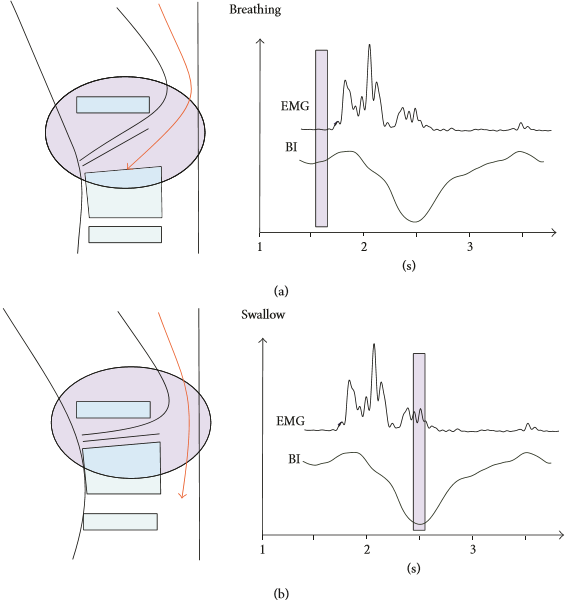
\includegraphics[width=7cm]
{Figure/EMGBIGraph}}
\caption{Illustration af, hvodan emg-og bioimpedans signaler opfører sig under vejrtrækning og mad/drikke indtagelse\cite{Schultheiss2014}}
\label{EMGBIGraph} 
\end{figure}
\pagebreak

Det biologiske væv, der skal måles kan illustreres som et elektrisk kredsløb, der består af tre elektriske komponenter (to modstande og en kondensator), se figur \ref{fig:vaevsmodel}. Den ene modstand i serie med en kondensator repræsenterer målregionens intracellulærvæske, hvorimod den anden modstand repræsenterer modstanden i ekstracellulærvæsken. I dette projekt sendes en konstant strøm med frekvens på 20 kHz igennem måleobjektets væv. I \nameref{bilag3} kan man læse, hvilken betydning frekvens størrelse har for måleresultatet. 
\begin{figure}[H]
\centering
{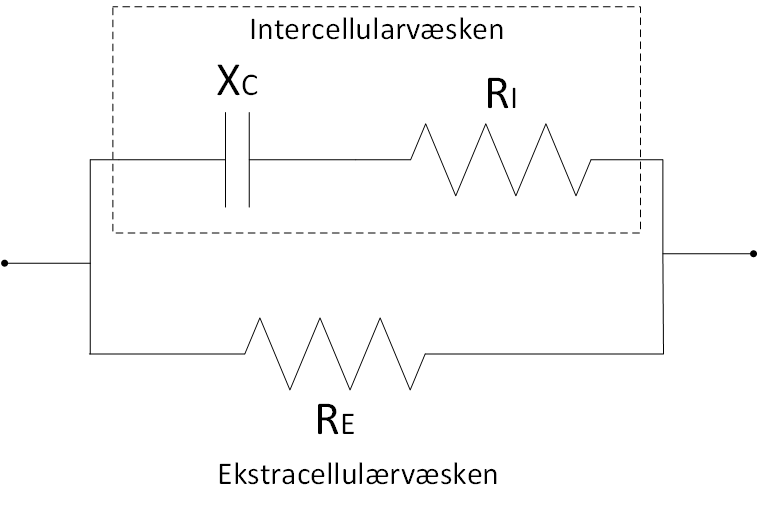
\includegraphics[width=10cm]
{Figure/vaevsmodel}}
\caption{Figuren viser et biologisk væv repræsenteret som et elektrisk kredsløb. Intracellulærvæsken består af modstanden  R\textsubscript{I} og kondensatoren X\textsubscript{C}, der har kapacitive egenskaber. R\textsubscript{E} er modstanden i ekstracellulærvæsken}
\label{fig:vaevsmodel}
\end{figure}
\section{Problemformulering}

Dette bachelorprojekt undersøger muligheden for at udvikle et device, der består af en BI-sensor og en EMG-sensor, der tilsammen kan monitorere og detektere synkefrekvensen. Devicet bliver fremover omtalt som Synkerefleksmonitor (SRM). Dette bachelorprojekt vil søge svar på følgende spørgsmål: 

\begin{itemize}
\item Kan man udvikle en prisbillig BI-sensor, der kan være alternativ til Fiber Endoskopisk Evaluering af Synkefunktionen (FEES) og Funktionel Videoradiologisk Evaluering af Synkefunktionen (FVES) til at undersøge synkefrekvensen på personer, der er ramt af dysfagi?
\item Kan man kombinere BI-sensor og EMG-sensor til måling af dysfagi?


\end{itemize}
Ved hjælp af primærlitteratur og sekundærlitteratur vil disse spørgsmål blive besvaret gennem dette projekt. 
\pagebreak

\section{Formål}

Formålet med dette bachelorprojekt er at udvikle et produkt, der består af en BI-sensor, der kan måle bioimpedans signaler, samt kombinere BI-sensor med en kommerciel EMG-sensor. Det overordnet system, der vil blive realiseret består af en BI sensor med elektroder, som er koblet til et raskt måleobjekt. Desuden kobles EMG-sensoren til måleobjektet med elektroder. En pc anvendes til processering og visning af data til et sundhedspersonale, se figur \ref{KonceptuelDiagram}.  

\begin{figure}[H]
\centering
{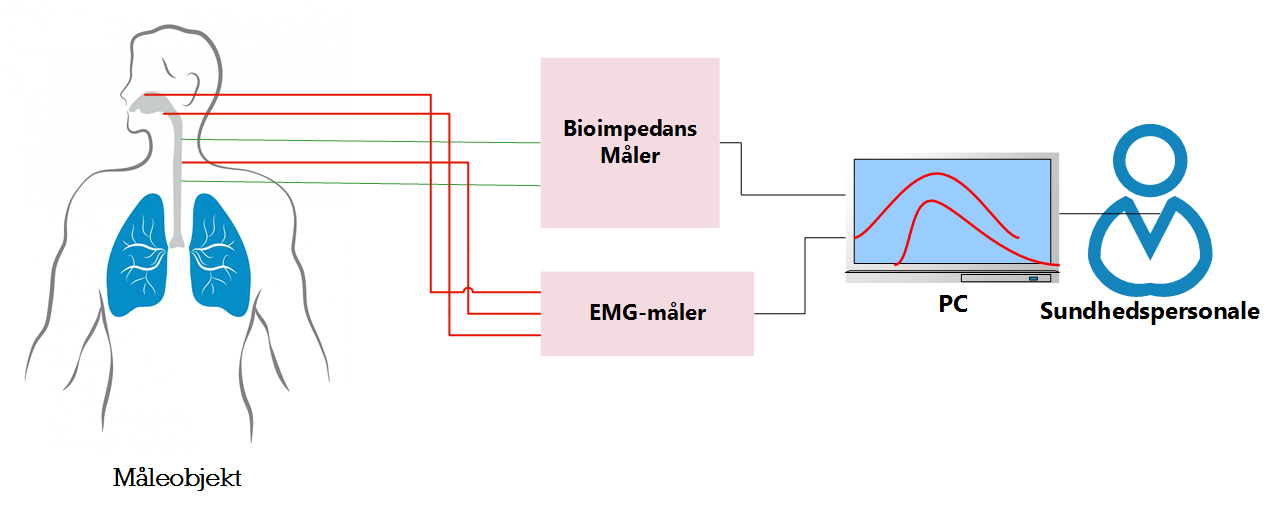
\includegraphics[width=11cm]
{Figure/KonceptuelDiagram}}
\caption{Illustration af  det overordnet system som dette projekt vil realisere}
\label{KonceptuelDiagram}
\end{figure}

Projektet vil fokusere på udvikling af den anbefalede prisbillig BI-sensor. Det er ligeledes projektets mål at genskabe de to signaler, der er vist på figur \ref{EMGBIGraph}. EMG-måleren bruges som supplerende redskab til BI-sensoren, da den kan detektere muskelaktiviteter, som finder sted før, under og efter et synk. Disse muskelaktiviteter er en forudsætning for, at synkningen kan ske. 

Det skal dog for god ordens skyld understreges at systemet, der realiseres i dette bachelorprojekt er på proof-of-concept stadie og må derfor ikke anvendes til kliniske undersøgelser. Det er ikke projektets mål at udvikle en endelig BI-sensor, der kan sættes i produktion eller anvendes til screening af personer med mistanke for dysfagi. 

\section{Projektdeltagere og hovedansvarsområder} 
Arbejdsfordelingen  mellem gruppemedlemmerne er fordelt ligeligt på grund af gruppens størrelse. Gruppen har valgt at dele projektet op i en software og hardwaredel, hvor alle i gruppen har ansvaret for  begge dele. Argumentet for den kollektive ansvarsfordeling er valgt, da gruppens medlemmer har vurderet, at en skarp opdeling af ansvarsområder vil medføre mindre koordinering og risiko for, at man isolere sig kun til sine ansvarsområder. Tabel \ref{Ansvarsfordeling} viser den valgte ansvarsfordeling. 

\begin{table}[H]
\centering

\begin{tabular}{|l|l|}
\hline
\textbf{Projektdeltagere}        & \textbf{Hovedansvarsområder}  \\ \hline
Mohamed Hussein Mohamed & Hardware \& Software \\ \hline
Martin Banasik          & Hardware \& Software \\ \hline


\end{tabular}

\caption{Indeholder gruppemedlemmernes navne og hovedansvarsområder }
\label{Ansvarsfordeling}
\end{table}


